\chapter{Testes e Resultados}

\vspace{-1.9cm}

Neste capítulo, são apresentados os resultados obtidos pelos programas propostos no capítulo anterior. Os dados medidos para cada programação são o tempo de execução, sendo que cada programa foi executado dez vezes para assim se obter os três menores tempos e a quantidade de \ac{LoC}.

\section{Compilando os Programas}

  Os programas em Java foram compilados com seu compilador padrão $javac$, conforme demonstrado a seguir:

  \begin{lstlisting}[mathescape=false]
  javac SomarNumeros.java
  javac FiltrarNumerosPares.java
  javac CalcularFactorial.java
  \end{lstlisting}

  Os programas em Scala foram compilados com seu compilador padrão $scalac$, conforme demonstrado a seguir:

  \begin{lstlisting}[mathescape=false]
  scalac SomarNumeros.scala
  scalac FiltrarNumerosPares.scala
  scalac CalcularFactorial.scala
  \end{lstlisting}

  Os programas em Clojure foram compilados através da ferramenta de compilação disponível para programas escritos em Clojure chamada Leiningen. Para compilar cada programa Clojure é necessário acessar a sua pasta e executar o comando:

  \begin{lstlisting}[mathescape=false]
  lein compile
  \end{lstlisting}

  O tempo de compilação do compilador Java leva vantagem quando comparado com os compiladores das linguagens Clojure e Scala. Por este motivo essas linguagens tem colocado muitos esforços para evoluir seu processo de compilação e torná-los mais rápidos. Um recurso que vem sendo incorporado pela linguagem Scala através da ferramenta SBT e pelo Clojure através da ferramenta LEIN, é a compilação incremental. Onde após uma primeira compilação completa do programa, as próximas compilações são realizadas apenas em arquivos que sofreram alterações.

  \section{Executando os Programas}

  Os programas em Java foram executados com seu interpretador padrão $java$ na mesma pasta onde cada programa foi compilado, conforme demonstrado a seguir:

  \begin{lstlisting}[mathescape=false]
  java SomarNumeros
  java FiltrarNumerosPares
  java CalcularFactorial
  \end{lstlisting}

  Os programas em Scala foram executados com seu interpretador padrão $scala$ na mesma pasta onde cada programa foi compilado, conforme demonstrado a seguir:

  \begin{lstlisting}[mathescape=false]
  scala SomarNumeros
  scala FiltrarNumerosPares
  scala CalcularFactorial
  \end{lstlisting}

  Os programas em Clojure foram executados através da ferramenta Leiningen. Para executar cada programa Clojure é necessário acessar a sua pasta e executar o comando:

  \begin{lstlisting}[mathescape=false]
  lein run
  \end{lstlisting}

\section{Resultados}

  \subsection{Tempo de Processamento}

    Todos os programas apresentaram os mesmo resultados, e o tempo de processamento utilizado foram os 3 menores de de 10 coletados para cada programa.

    \begin{table}[htb] % [htb]-> here, top, bottom
       \centering   % tabela centralizada
       \large       % tamanho da fonte
       \setlength{\arrayrulewidth}{2\arrayrulewidth}  % espessura da  linha
       \setlength{\belowcaptionskip}{10pt}  % espaço entre caption e tabela
       \caption{\it Tempo (ms) de Processamento Gasto Por Cada Programa}
       \begin{tabular}{|l|r|r|r|} % c=center, l=left, r=right
          \hline
          Programa (Tentativa) & Java & Clojure & Scala \\
          \hline \hline
          Somar Números Inteiros (1) & 4.815872 ms & 6.564096 ms & 1.544192 ms \\
          \hline
          Somar Números Inteiros (2) & 4.71808 ms & 6.727168 ms & 1.579008 ms \\
          \hline
          Somar Números Inteiros (3) & 4.827136 ms & 6.550016 ms & 1.607936 ms \\
          \hline
          Manipulação de Listas (1) & 78.750976 ms & 0.175872 ms & 17.15712 ms \\
          \hline
          Manipulação de Listas (2) & 79.156992 ms & 0.180992 ms & 17.278208 ms \\
          \hline
          Manipulação de Listas (3) & 78.694144 ms & 0.178944 ms & 17.127936 ms \\
          \hline
          Cálculo Fatorial (1) & 1.179136 ms & 1.050112 ms & 0.84608 ms \\
          \hline
          Cálculo Fatorial (2) & 1.181952 ms & 1.041920 ms & 0.866048 ms \\
          \hline
          Cálculo Fatorial (3) & 1.180928 ms & 1.049088 ms & 0.851968 ms \\
          \hline
       \end{tabular}
    \end{table}

    Os melhores (menores) tempos de cada programa em cada linguagem de programação foram utilizados para compor o gráfico a seguir.

    \begin{grafico}[H]
      % Alterar espaçamentos antes e depois do caption
      \setlength{\abovecaptionskip}{5pt}
      \setlength{\belowcaptionskip}{0pt}
      % Caption
      \caption[Tempo de processamento gasto por cada linguagem de programação]
        {Tempo de processamento gasto por cada linguagem de programação}
      \centering
      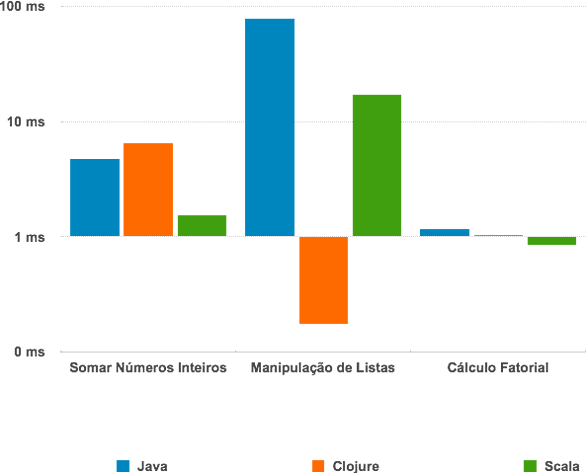
\includegraphics[width=1\textwidth]{imagem/graficos/grafico-programas.png}
      % Caption centralizada
      \captionsetup[grafico]{justification=centering}
      % Fonte
      \captionfont{\small{\textbf{\\Fonte: Dados da pesquisa}}}
    \end{grafico}

  \subsection{Linhas de Código}

    Para analisar a legibilidade de cada programa foi utilizado a quantidade de linhas de código como uma medida. As linhas que não continham nenhum caractere não foram acrescentadas a tabela a seguir.

    \begin{table}[htb] % [htb]-> here, top, bottom
       \centering   % tabela centralizada
       \large       % tamanho da fonte
       \setlength{\arrayrulewidth}{2\arrayrulewidth}  % espessura da  linha
       \setlength{\belowcaptionskip}{10pt}  % espaço entre caption e tabela
       \caption{\it Linhas de Código Utilizada Por Cada Programa}
       \begin{tabular}{|l|r|r|r|} % c=center, l=left, r=right
          \hline
          Programa & Java & Clojure & Scala \\
          \hline \hline
          Somar Números Inteiros & 12 & 10 & 9 \\
          \hline
          Manipulação de Listas & 16 & 10 & 8 \\
          \hline
          Cálculo Fatorial & 16 & 13 & 10 \\
          \hline
       \end{tabular}
    \end{table}

    Os melhores (menores) tempos de cada programa em cada linguagem de programação foram utilizados para compor o gráfico a seguir.

    \begin{grafico}[H]
      % Alterar espaçamentos antes e depois do caption
      \setlength{\abovecaptionskip}{5pt}
      \setlength{\belowcaptionskip}{0pt}
      % Caption
      \caption[Linhas de código por cada linguagem de programação]
        {Linhas de código por cada linguagem de programação}
      \centering
      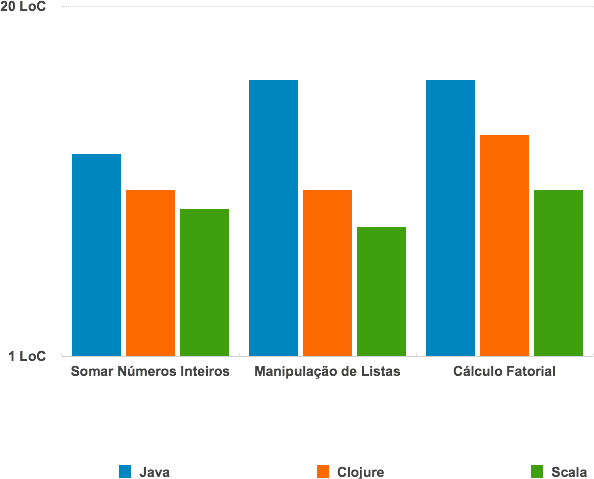
\includegraphics[width=1\textwidth]{imagem/graficos/grafico2-programas.png}
      % Caption centralizada
      \captionsetup[grafico]{justification=centering}
      % Fonte
      \captionfont{\small{\textbf{\\Fonte: Dados da pesquisa}}}
    \end{grafico}
